\documentclass{rapport}

\newcommand{\mysql}{\textit{MySQL}}

\title{Rapport de Spécifications}

\begin{document}

	\begin{titlepage}
		\begin{sffamily}
			\begin{center}
				
				% Upper part of the page. The '~' is needed because \\
				% only works if a paragraph has started.
				
\includegraphics[width=400pt]{logo_INSA.png}~\\[2.5cm]
				
				\textsc{\huge Rapport de pré-étude}\\[2.5cm]
				
				% Title
				\HRule \\[0.4cm]
				{ \huge \bfseries Système de gestion informatisée des mobilités\\[0.4cm] }
				
				\HRule \\[4cm]
				
				% Author and supervisor
				\begin{minipage}{0.4\textwidth}
					\begin{flushleft} \large
						\emph{Étudiants :}\\
						Jean \textsc{Chorin}\\
						Damien \textsc{Duvacher}\\
						Aurélien \textsc{Fontaine}\\
						Étienne \textsc{Geantet}\\
						Thomas \textsc{Hareau}\\
						Arnaud \textsc{Martin}\\
					\end{flushleft}
				\end{minipage}
				\begin{minipage}{0.5\textwidth}
					\begin{flushright} \large
						\emph{Encadrants :} \\
						Nikolaos \textsc{Parlavantzas}\\
						Christian \textsc{Raymond}
					\end{flushright}
				\end{minipage}
				
				\vfill
				
				% Bottom of the page
				{\large Année 2015 - 2016}
				
			\end{center}
		\end{sffamily}
	\end{titlepage}
	\tableofcontents
	
	\chapter{Introduction}

Notre projet a pour but la création d'une plateforme de gestion des mobilités de l'INSA de Rennes. Celle-ci facilitera l'affectation et le suivit des élèves en mobilité sortante. Elle permettra aussi une meilleure traçabilité des élèves, et l'obtension de données statistiques.

Vous pourrez retrouver le choix des technologies et les spécifications fonctionnelles de notre projet dans les précédents rapports. Pour rappel, notre application Web est développée en \php, à l'aide du framework \symfony. Elle utilise le système de base de données \mdb et est hébergée au Centre de Ressources Informatiques (CRI) sur un serveur \textit{Nginx}. Nous utilisons enfin le système CAS (Central Authentication Service) du CRI pour nous permettre d'authentifier les utilisateurs.

\bigbreak

Notons que notre application est déjà en cours d'utilisation. En effet, nous avions pour objectif de développer notre projet en parallèle à la gestion des mobilités de cette année. Nous avions donc des contraintes de temps plus fortes, mais aussi de quoi tester notre application en situation réelle. Elle a ainsi été utilisée pour affecter les élèves de 3A et 4A du département informatique cette année. Nous en sommes désormais à l'implémentation de la gestion des documents nécessaires aux mobilités (notamment contrats d'étude).

\bigbreak

L'architecture de notre projet sera séparé en deux parties. Nous verrons d'abord la partie base de données, puis l'organisation des vues du site. Nous verrons ensuite comment s'articulent les différents modules utilisés.

\bigbreak
La figure \ref{useCase} est un rappel du fonctionnement habituel de l'application, et l'avancement du projet par la même occasion. Notons que les fonctionnalités en rouge ne sont pas encore implémentées, et que celles en vert sont en cours d'implémentation ou de test. 

\begin{figure}
	\centering
	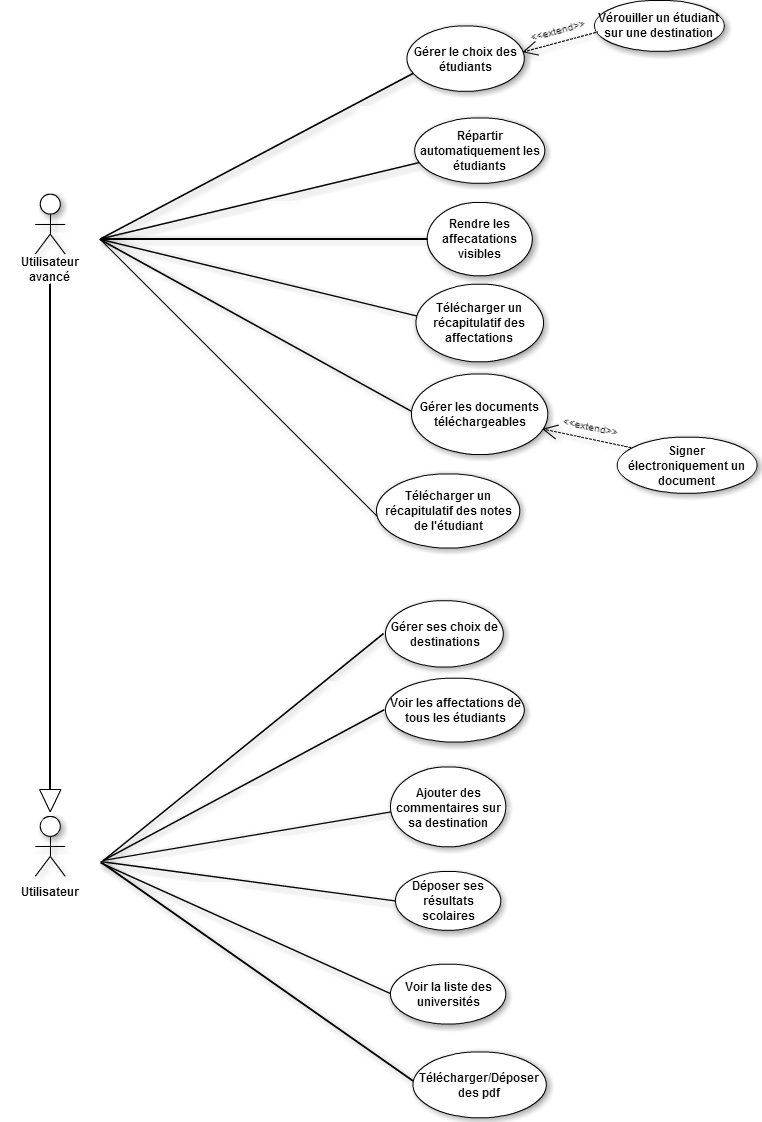
\includegraphics[scale=0.7]{images/useCaseDiagram.png}
	\caption{Diagramme de cas d'utilisation de l'application}
	\label{useCase}
\end{figure}
	
	
	\chapter{Le projet}
	 Lors de leur 4\ieme{} année d'étude, les étudiants de l'INSA de Rennes doivent réaliser un projet. Notre groupe a choisi %lol
	  le sujet \og Système de gestion informatisé des mobilités \fg. Nous allons donc développer une application facilitant le traitement des étudiants et de réduire la perte de papier due aux nombreuses impressions nécessaires.

		Ceci est la page d'entrée du site pour les élèves. Une fois identifiés via le CAS, ils sont dirigés vers une page qui est propre à chaque élève et qui se modifie selon ses choix.
Sur cette page est présent :

		\input{Etudiant/Page d'accueil étudiant étape 2}
		\input{Etudiant/Page d'accueil étudiant étape 3}
		\input{Etudiant/Voeux Etudiants}
		
	
	\chapter{Le projet}
	 Lors de leur 4\ieme{} année d'étude, les étudiants de l'INSA de Rennes doivent réaliser un projet. Notre groupe a choisi %lol
	  le sujet \og Système de gestion informatisé des mobilités \fg. Nous allons donc développer une application facilitant le traitement des étudiants et de réduire la perte de papier due aux nombreuses impressions nécessaires.

		\input{Universités/Liste universités}
		\input{Universités/Fiche université}
		
	
	\chapter{Le projet}
	 Lors de leur 4\ieme{} année d'étude, les étudiants de l'INSA de Rennes doivent réaliser un projet. Notre groupe a choisi %lol
	  le sujet \og Système de gestion informatisé des mobilités \fg. Nous allons donc développer une application facilitant le traitement des étudiants et de réduire la perte de papier due aux nombreuses impressions nécessaires.

	 \input{Admin/Page d'accueil admin}
	 \section{Algorithme d'affectation}
\label{sec::moulinette}

\begin{figure}[H]
	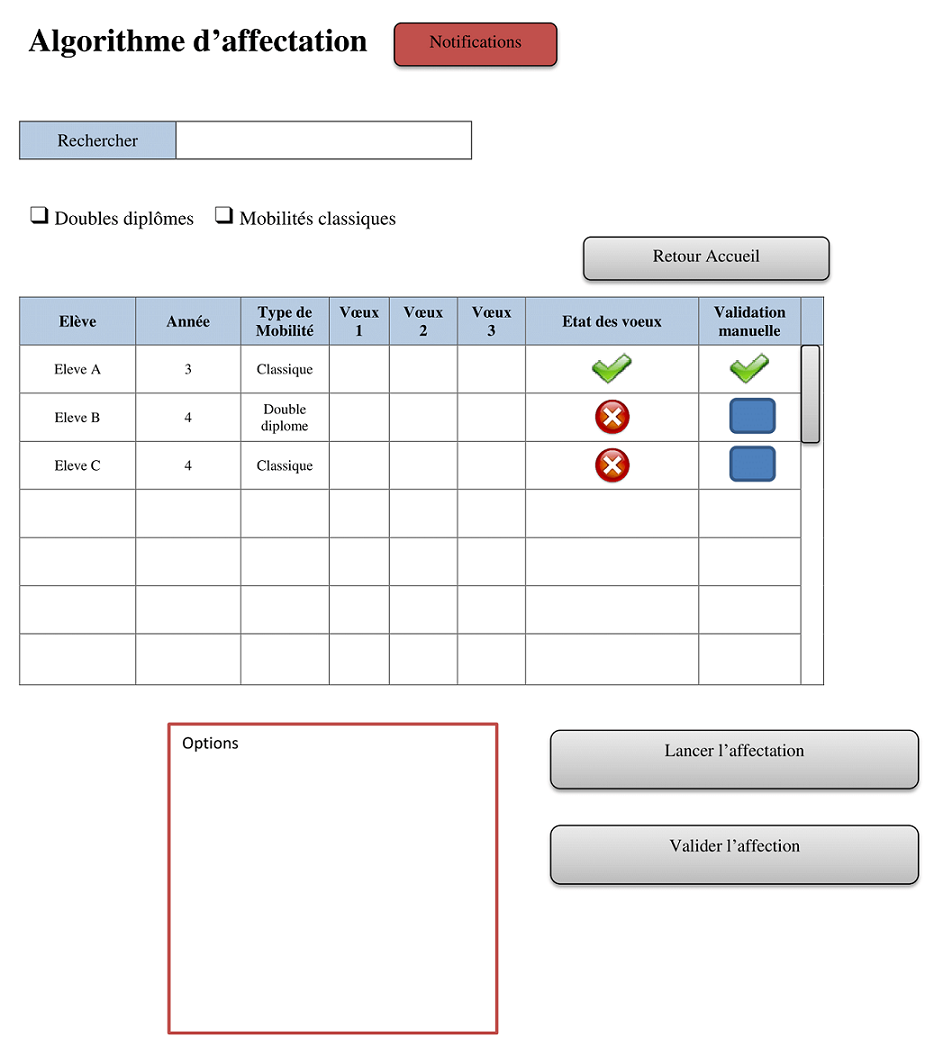
\includegraphics[scale=0.7]{Admin/Moul.png}
	\caption{Page de gestion de l'algorithme d'affectation}
	\label{fig::moulinette}
\end{figure}

La figure \ref{fig::moulinette} présente la page sur laquelle se trouve un tableau récapitulant les vœux définitifs des élèves, après la fin des choix de vœux (phase 1). Ce tableau comprend donc la liste des élèves, leur année, la liste des vœux, le type de mobilité choisie (double diplôme, mobilité classique), leur état (validé, à validé).

Encore présent sur ce tableau; une zone de recherche par mot clé ainsi que plusieurs filtres (années, universités, type de mobilité...).

\bigbreak

L'administrateur peut, sur cette page, gérer les paramètres de l'algorithme avant de le lancer (ajout de paramètres particuliers modifiant l'ordre d'attribution des vœux, en plus des notes).

\bigbreak

Il est aussi possible à l'administrateur de valider les vœux d'un élève manuellement. Cela fait sortir cet élève de la liste des élèves concernés par l'algorithme (il apparaitra toujours dans la liste des élèves mais son état deviendra "validé" et il ne sera pas pris en compte par l'algorithme).

\bigbreak

Enfin, un bouton permettant de lancer l'algorithme d'attribution des vœux. Lorsque l'algorithme est terminé, la phase 1 est finie et la phase 2 est lancée. Cela signifie que les différentes vues deviendrons celles de la phase 2.
	 \input{Admin/Page d'accueil SRI}
	 
	\chapter*{Conclusion}
\addcontentsline{toc}{chapter}{Conclusion}	

Au terme de cette étape, nous avons défini un premier design de notre application, en expliquant les fonctionnalités offertes aux utilisateurs. 
Les chapitres \ref{chap::etudiants} et \ref{chap::admins} présentent l'interface offerte à chaque type d'utilisateur par notre application. Le chapitre \ref{chap::universites} explique comment les utilisateurs accèderont aux informations sur les universités.
Enfin, le chapitre \ref{chap::archi_logicielle} présente succinctement l'architecture logicielle de notre application.
Nous pouvons aussi présenter une ébauche des vues accessibles, bien que l'apparence même soit sans doute sujette à changement.
\bigbreak
Nous allons désormais travailler à l'implémenter puis tester un premier prototype fonctionnel. Celui-ci répondra à la première étape d'un cycle de départ en mobilité, c'est-à-dire les vœux des étudiants puis leur affectation. L'objectif étant d'avoir à disposition une version incomplète mais fonctionnelle de l'application, pour la tester en situation réelle courant Décembre. 
	
\end{document}

